\subsection{Frequenzmessung}\label{subsec:Frequenzmessung}
Um die Genauigkeit der Frequenzmessung zu bestimmen, testeten wir das Theremin bei den  Frequenzen aus der Tabelle \ref{tab:Toene_Frequenzen} in Kapitel \ref{subsec:Musiktheorie}.
 Wir verwendeten dazu anstatt unseres PCB einen Funktionsgenerator, da keine genaue Messung mit dem PCB möglich ist. Um die Frequenz auszulesen, nutzten wir das Tool \textit{SignalTap Logic Analyzer} in Quartus um auf das Register der Frequenzmessung mit den Messresultaten zuzugreifen.
 Zu Beginn der Messung war eine Bestimmung des Offset des Referenzoszillator nötig. Dazu wurde der Frequenzgenerator um \SI{120}{Hz} tiefer eingestellt als der Referenzoszillator. Da \SI{120}{Hz} die Frequenz ist auf die Kalibriert wird. Daraus ergab sich ein Offset von  \SI{6}{Hz}.
 Für die Bestimmung der minimal und maximal gemessenen Frequenzwerte haben wir uns dafür entschieden aus dem SignalTap 20 Werte auszulesen. Aus dem Maximum und Minimum bestimmten wir die grösste Abweichung zum entsprechenden Ton. Aus diesen Abweichungen berechneten wir die Werte aus Abbildung \ref{img:plot_frequenzmessung} .

 Alle gemessenen Werte liegen unter einem Fehler von 8 Cent. Wie bereits im Kapitel \ref{subsec:Musiktheorie} beschrieben, ist es schwer zu sagen, wann ein Ton als ''nicht getroffen`` empfunden wird. Daher haben wir uns darauf geeinigt, dass Werte unter 8 Cent als ''getroffen`` empfunden wird. Somit erfüllen alle Frequenzen diese Genauigkeit.
 
 Wie in Abbildung \ref{img:plot_frequenzmessung} ersichtlich ist, steigt die Messung mit zunehmender Frequenz immer mehr an. Dies spricht mit der Simulation aus Matlab aus Abbildung \ref{img:plot_freq_sim} überein. Dabei wurde in Matlab dieselbe Messmethode Simuliert in \SI{1}{Hz} schritten von \SI{100}{Hz} bis \SI{2}{kHz} Auch die tiefen Cent Werte um \SI{600}{Hz} stimmen mit der Simulation überein, da gewisse Frequenzen mit der gewählten Abtastfrequenz von \SI{1.2}{MHz} eine genauere Messung ergeben.
 \begin{figure}[h]
 	\centering
 	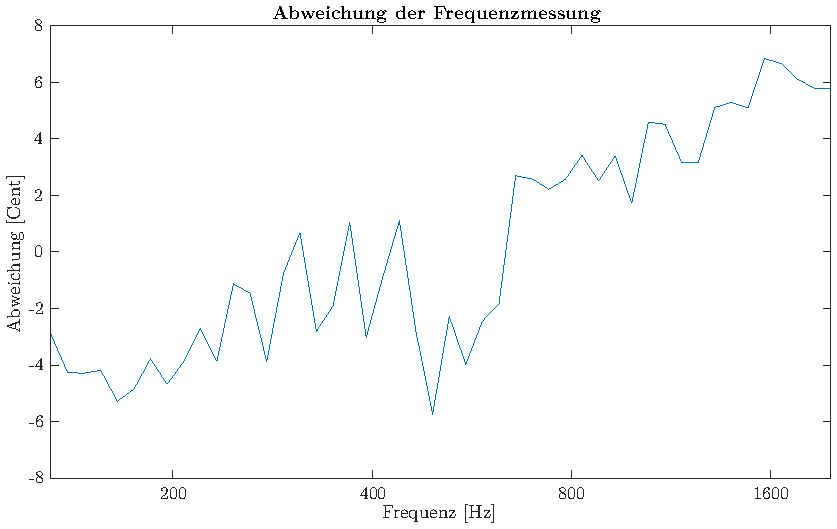
\includegraphics[width=0.9\textwidth]{Validierung_frequenzmessung.pdf}
 	\caption{Maximale Abweichung der Frequenzmessung.}
 	\label{img:plot_frequenzmessung}
 \end{figure}
 \begin{figure}[h]
	\centering
	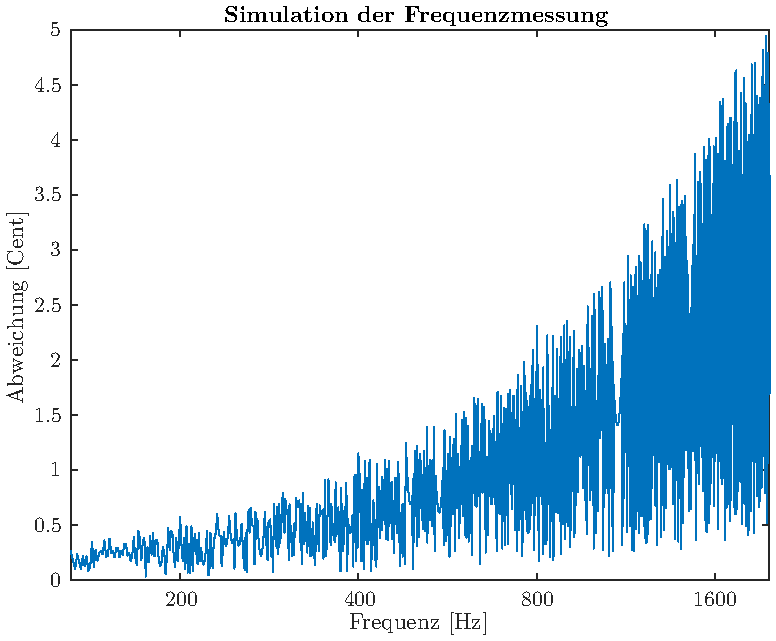
\includegraphics[width=0.9\textwidth]{Simulation_Frequenzmessung.pdf}
	\caption{Abweichung der Frequenzmessung in der Simulation}
	\label{img:plot_freq_sim}
\end{figure}
\begin{table}[H]
	\centering
	\caption{Verwendete Messmittel}
	\label{tab:Verwendete_Messmittel_freq}
	\begin{tabular}{l|l}
		\textbf{Messgerät} & \textbf{Bezeichnung}	\\
		\hline \hline
		
		Funktionsgenerator  & MSZ-M-0051   \\ 
		&        \\ 
		\hline
		SignalTap Logic Analyzer  &    \\ 
		&        \\ 
			\hline
	\end{tabular}
\end{table} 

\pagebreak
